%% -*- mode: latex; mode: flyspell -*-
\documentclass[12pt, letter]{article}

%% Class name and Assignment number
%%
\newcommand{\courseName}{ECE435 Medical Image Processing}
\newcommand{\assignName}{Progress Report}
    
%% Packages
\usepackage{amsmath,amsfonts,amssymb,amsthm,dsfont}
\usepackage{graphicx}
\usepackage[bookmarks=false]{hyperref}
\usepackage{color}
\usepackage{listings}
\usepackage{color}
\usepackage{amsmath}
\usepackage{subfig}
\usepackage{multirow}
\usepackage{subfig}

\lstset{
    showstringspaces=false,
    basicstyle=\ttfamily,
    keywordstyle=\color{blue},
    commentstyle=\color[grey]{0.6},
    stringstyle=\color[RGB]{255,150,75}
}

\newcommand{\inlinecode}[2]{\colorbox{lightgray}{\lstinline[language=#1]$#2$}}

%% Paper format
\usepackage{geometry}
\geometry{
    letterpaper,
    %% total={216mm,279mm}, %< NSERC size
    margin=2.00cm,     %< default
    %% margin=1.87cm,       %< NSERC tightest
}

%% Headers and footers
\usepackage[explicit]{titlesec}
\newpagestyle{titlesec_assignment}{
  \sethead{\courseName}{}{\assignName}\setfoot{}{\thepage}{}
  \headrule
  %% \footrule
}

\begin{document}
%% Set header and footer
\pagestyle{titlesec_assignment}

%% Title
\title{\courseName\\\assignName}
\author{Brian Pattie, Yiping Wang}
\maketitle

%% Abstract
%\abstract{The project proposal is to be submitted as one pdf file, containing: }

%% Content

\section{Introduction}

%stating the title of the project and the dataset that you are working with
Our team choose the MICCAI 2013 paper, Automated Nucleus and Cytoplasm Segmentation of Overlapping Cervical Cells \cite{main}, to work with. The title of our project is, ``Segmentation of the Overlapping Cervical Cells by Joint Level Set Method". 

The Cell Segmentation in Cervical Cytology dataset, ISBI 2014, provides 16 Extended Depth of Field (EDF) real cervical cytology images and 945 synthetic images. It provides enough high-quality training and testing synthetic images, of 45 training and 90 testing images are annotated by the expert. The rest of 810 synthetic data will be used for evaluation. 


\section{Summary of the Chosen Paper}
The paper's primary contribution is an application of the Joint Level Set Method (LSM), which is described in the next section. This section will instead focus on the scene segmentation steps which set up the segmentation of overlapping cells.

The first step is an one-pass EDF algorithm. The ISBI 2014 database features only real images with EDF already applied and synthetic images for which it is not necessary, so this step will be skipped in our implementation.

The second step is the segmentation of cell clumps.  Quick-shift, a mode seeking algorithm, is applied to the image to create a super-pixel map. This divides the image into connected areas that share the same grey-level value. This reduces noise, and produces very clean edges. An edge detector is applied to the super-pixel map to create an edge map. The paper does not specify what edge detector is used, so we will be using Canny edge detection. A convex hull is built around the connected components of the edge map. The effect is a rough division between cell clump pixels that fall inside cell clumps, and pixels belonging to the background. These initial assignments are used by an unsupervised binary classifier which will reclassify each pixel as either "Cell Clump" or "Background".

The third step is the detection and segmentation of cell nuclei using a Maximally Stable Extremal Regions (MSER) algorithm. This relies on the assumption that nuclei will be near-circular in shape and appear as a darker grey than the surrounding cytoplasm.

\section{Level Set Method for Image Segmentation}
\subsection{Introduction}
Segmentation is defined as partitioning portions of an image. It adds structure to a raw image. In the case of medical imaging, segmentation can involve identifying which portion of an image is a tumor, or separating white matter from gray matter in a brain MRI scan. 

The chosen paper proposed a novel Joint LSM algorithm for accurately segmenting the individual cytoplasm and nuclei from a clump of overlapping cervical cells. Though the mathematics derivation involved and difficult for us to grasp in such a short time, we will discuss the fundamental idea of LSM, and how can it be used for image segmentation, which is an essential step for us to understand the algorithm proposed by the paper. 

The segmentation problem boils down to finding curves to enclose regions of interest. Explicitly and intuitively, we can model the curves by sampling enough points on the curves. However, there are some drawbacks involved in updating the sampling points. For example, if two separate closed curves need to merge into one, or one needs to be split in two, when would this merge or split take place? How would an algorithm to detect when to merge or split? Suppose we have came with an algorithm to detect when and where the sampling points are going to merge or split, the data structure for the curve(s) would then need to be updated as well. The explicitly modeling requires lot of manually tracking and is not easy to implement. Fortunately, these difficulties can be alleviated using the LSM. 

The LSM was first presented by Osher and Sethian for front propagation, being applied for models of ocean waves and burning flames. Malladi first applied LSM to medical imaging purposes. The idea behind the LSM is to embed a curve within a surface. For example, we can embed a two-dimensional curve within a three-dimensional surface. By implicitly modeling curves in this way, the above mentioned problems of merging and splitting are addressed without special treatment. 

\subsection{Formulation}
Suppose we have a surface $\phi(x)$. The $c$-level set of the surface is given by:
\begin{equation}
    \{x \mid \phi(x) = c\}
\end{equation}

To track the contour, we evolve the surface by rising, falling, expanding, shrinking, etc. Therefore, it is sufficient to track the level curve at $c = 0$, which is the zero level set of $\phi$
\begin{equation}
    \{x \mid \phi(x) = 0\}
\end{equation}

As we are dealing with surface evolution, we can parameterize the surface with a temporal variable $t$ such that:

\begin{equation}
    \phi(x(t), t) = 0
\end{equation}{}

where $x(t)$ represents the positions on the $xy$-plane at time $t$.

Since we want to track the movement of the zero level curve of $\phi$, we will derive it with respect to $t$, i.e., we derive the equation of the motion of $\phi$:

\begin{equation}
    \frac{\partial \phi(x(t), t)}{\partial t} = 0
\end{equation}

By Chain Rule,

\begin{equation}
    \frac{\partial \phi}{\partial x(t)} \frac{\partial x(t)}{\partial t} + \frac{\partial \phi}{\partial t} = 0
\end{equation}

or in Leibniz form,

\begin{equation}
    \nabla \phi x_t + \phi_t = 0
\end{equation}

The direction of the curve's movement is the unit vector of the gradient of the surface, which is $\frac{\nabla \phi}{\left\Vert \nabla \phi \right\Vert}$. Since there will exist a force to move the curve, we denote it as $F$. Hence, the speed vector is given by $x_t = F \frac{\nabla \phi}{\left\Vert \nabla \phi \right\Vert}$.

After some algebra, we drive the surface evolution with respect to time $t$,

\begin{equation}
    \phi_t = -F \left\Vert \nabla \phi \right\Vert
\end{equation}

To solve $\phi$, we use the Finite Difference Method to approximate the solution.  

\begin{equation}
    \frac{\partial \phi(x(t), t)}{\partial t} = \frac{\phi(x(t) + \Delta t) - \phi(x(t), t)}{\Delta t}
\end{equation}

or in Leibniz form.

\begin{equation}
    \frac{\partial \phi(x(t), t)}{\partial t} = \frac{\phi(x(t) + \Delta t) - \phi(x(t), t)}{\Delta t}
\end{equation}

After some algebra,

\begin{equation}
    \phi ' (x(t), t + \Delta t) = \phi (x(t), t) + \Delta t F \left\Vert \nabla \phi \right\Vert
\end{equation}

where $\phi '$ represents the the surface evolution after time $\Delta t$.

\subsection{Image Segmentation}
The gradient of the image can be used for edge detection. The magnitude of the gradient gives the amount of the difference between pixels in the neighborhood, i.e., the strength of the edge. The gradient orientation gives the direction of the greatest change. which is the direction across the edge, i.e., the edge normal. 

In Equation $(10)$, $F$ is intuitively a force that drives curve propagation. In other words, we can think of $F$ as a velocity field, which every vector gives the direction and magnitude of the surface $\phi$. As $F$ is the velocity field and we want the magnitude of $F$ to be high at all regions that are not the border of the object of interest, and low otherwise. Put simply, we want the curve to propagate quickly in the background of the image, and propagate slowly or even stop at the edge of the object. 

One way to model $F$ is using the edge detector since it provides the properties we need. The gradient in the edge of object is the largest and slower in other places. Therefore, the inverse of the edge detector has the lowest propagation magnitude at the border of the object and larger propagation magnitude elsewhere. 

\begin{equation}
    F = g(I) = \frac{1}{1 + \left\Vert \nabla I \right\Vert^2}
\end{equation}

Hence, we can iterate the Finite Method Difference equation with $F$ defined in (11) hundreds of times to approximate the surface $\phi$. 

Figure~\ref{fig:lsm_demo} shows the implementation of the above algorithm on a cervical cell. We can see the shape of the cervical cell is preserved.

\begin{figure}%
    \centering
    \subfloat[Cervical Cells Before Applying LSM]{{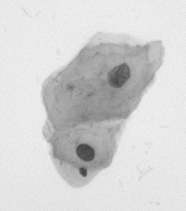
\includegraphics[width=7cm]{images/cell_before_seg.png}} }%
    \qquad
    \subfloat[Cervical Cells Before Applying LSM]{{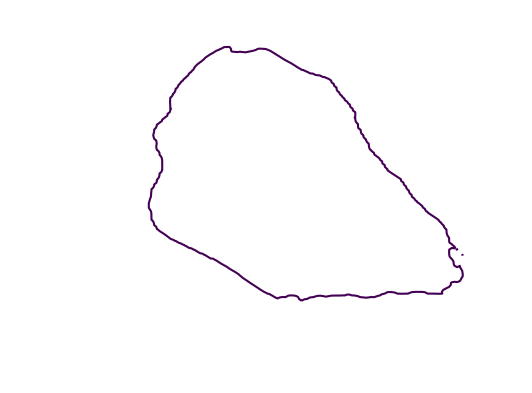
\includegraphics[width=7cm]{images/cell_after_seg.png}} }%
    \caption{Apply the Naive LSM to a Cervical Cell}%
    \label{fig:lsm_demo}%
\end{figure}

Since the above algorithm are the most naive LSM for image segmentation, it only works for images containing clearly separated object(s). For our project, by using advanced level set algorithm,  i.e., Joint LSM, as proposed in the paper \cite{main}, we are able to segment overlapping cells. 

\section{Preliminary Results}
%Preliminary results regarding implementation of the algorithm described in the paper

As of this point, we have developed MATLAB Code that will perform the first few steps of the cell segmentation process. For ease of understanding and implementation, we elected to use a Mean-shift algorithm instead of the Quick-shift algorithm used by the paper's authors. Our naive Mean-shift algorithm takes four parameters: \textit{M, i, v, iter}. \textit{M} is the image, which is expected to be in 8-bit unsigned integer format. Pixels within radius \textit{r} and greyscale value \textit{v} will contribute to the mean. The algorithm performs \textit{iter} iterations on \textit{M} and returns the resulting super-pixel map. We run a Canny edge detector on the super-pixel map to get an edge map that will later be used for drawing the convex hulls that initialize the binary classifier. Figure~\ref{fig:mean_shift} compares the results of the Mean-shift to the original image. Figure~\ref{fig:canny} shows the Canny edge detector result. 

\begin{figure}%
    \centering
    \subfloat[Original Overlapping Cervical Cells]{{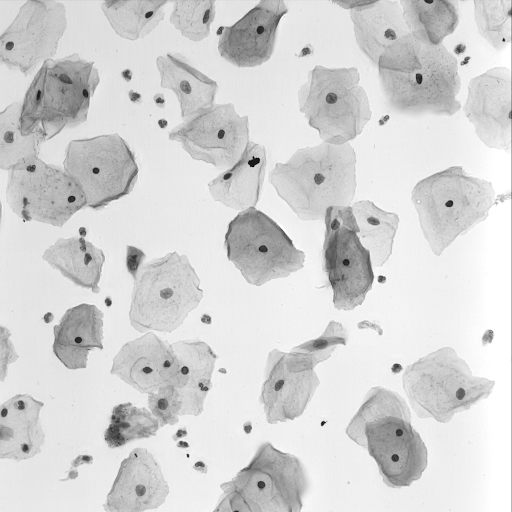
\includegraphics[width=7cm]{images/origin.png}} }%
    \qquad
    \subfloat[After Mean-shift Pre-processing]{{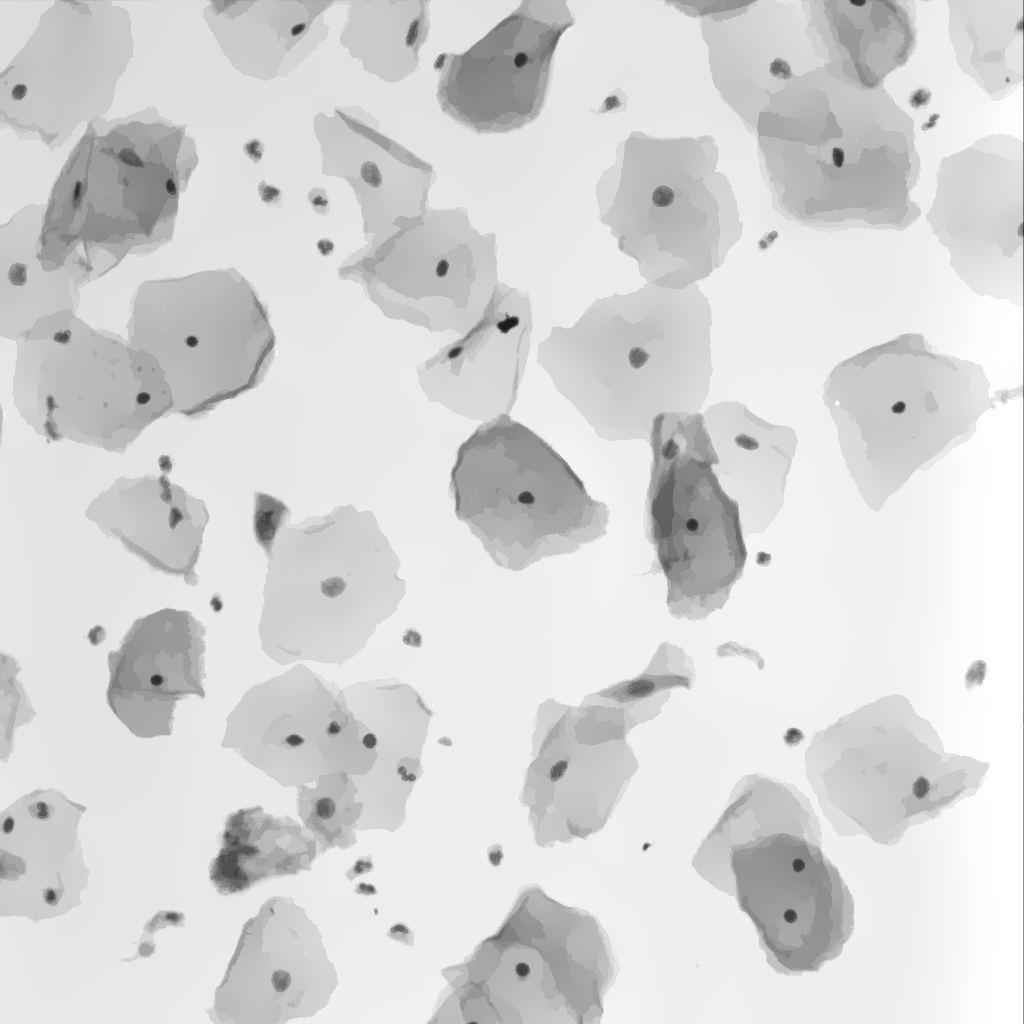
\includegraphics[width=7cm]{images/mean_shift.png}} }%
    \caption{Comparison of Mean-shift Output to Original Image}%
    \label{fig:mean_shift}%
\end{figure}

\begin{figure}%
    \centering
    \subfloat[Original Overlapping Cervical Cells]{{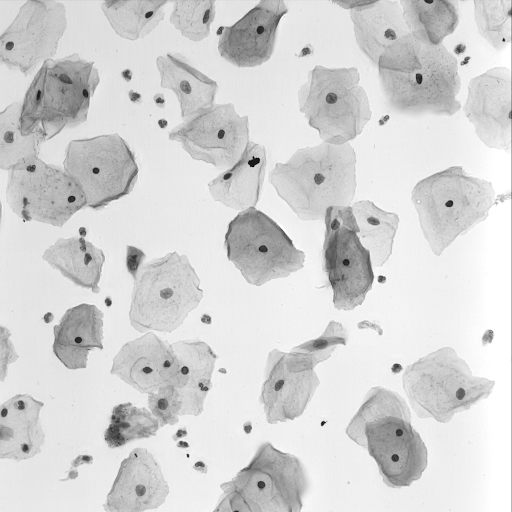
\includegraphics[width=7cm]{images/origin.png}} }%
    \qquad
    \subfloat[After Mean-Shift and Canny Edge Detector]{{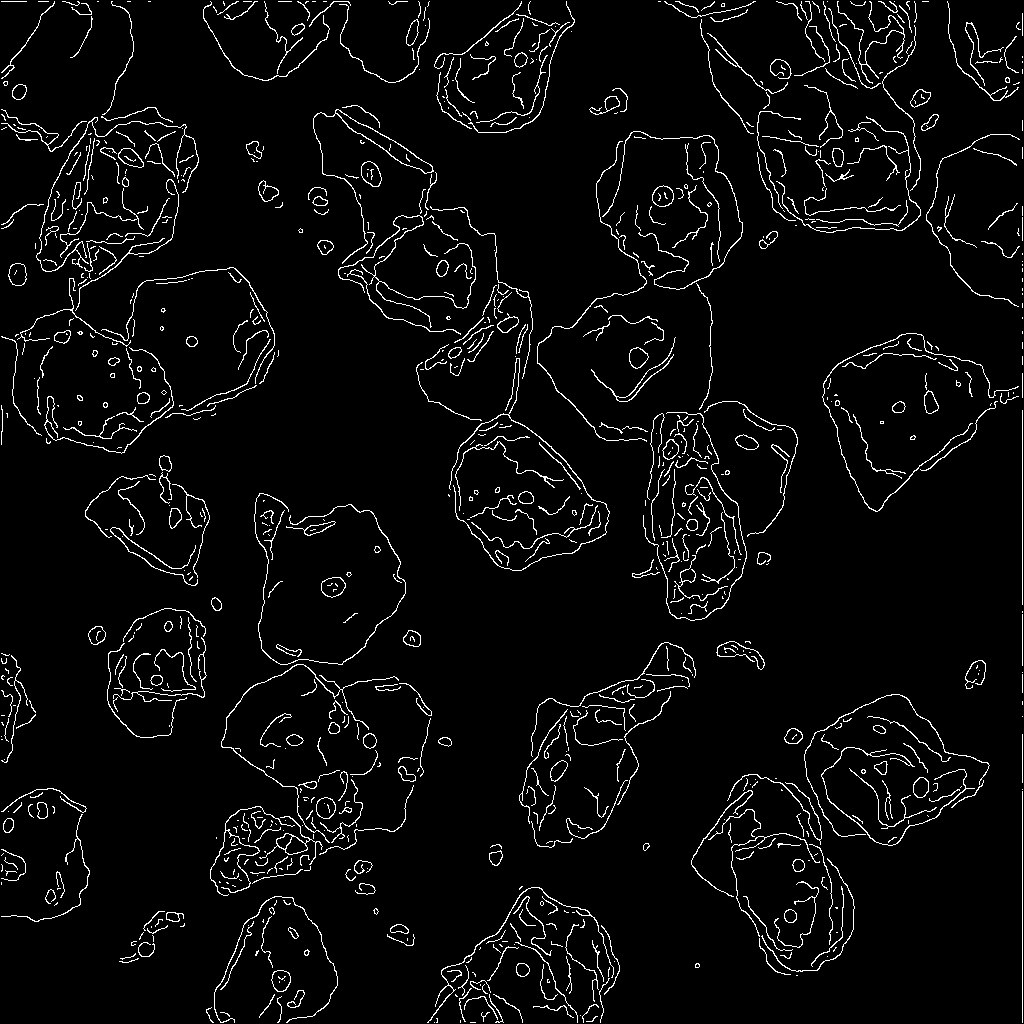
\includegraphics[width=7cm]{images/canny.png}} }%
    \caption{Comparison of Edge Map to Original Image}%
    \label{fig:canny}%
\end{figure}


\section{Project Management}
%intermediate and final milestones, estimated challenges, distribution of workload among team members (if applicable).

With Mean=shift and edge detection complete, we can move on to the next step which is generating the convex hulls to be used by the unsupervised binary classifier to classify "background" and "cell clump" pixels.

The primary contribution of this paper is an involved and intractable mathematics derivation, we anticipate that this would be the most difficult part for us to understand. Moreover, the implementation of the Joint LSM would also be a challenge for us.

We may run into accuracy issues due to the use of Mean-shift over Quick-shift. It appears at this point that the clean edges made possible by Mean-shift should fulfill our needs, but the nuclei may not have been sufficiently averaged for the MSER algorithm.


Table~\ref{tab:milestones} describes our tentative milestones.


\captionof{table}{Tentative Milestones} \label{tab:milestones} 
\centering
\begin{tabular}{ |l|l|l| }
	\hline
	\multicolumn{3}{ |c| }{Project Milestones} \\
	\hline
	Assignee & Tasks & Deadline \\ \hline
	\multirow{1}{*}{Yiping Wang} & Unsupervised binary classifier & March 17th \\ \hline
	\multirow{1}{*}{Brian Pattie} & Segmentation of Nuclei via MSER & March 17th \\ \hline
	\multirow{1}{*}{Both} & Joint Level Set Segmentation & March 24th \\ \hline
	\multirow{1}{*}{Both} & Oral Presentation Slides & March 30th \\ \hline
	\multirow{1}{*}{Both} & Finalize Code & April 6th \\ \hline
	\multirow{1}{*}{Both} & Video Demo & April 8th \\ \hline
	\multirow{1}{*}{Both} & Final Report & April 11 \\ \hline
\end{tabular}

\bibliographystyle{plain}
\bibliography{citation-260127853}

\end{document}